\documentclass{article}
\usepackage{graphicx} % Required for inserting images
\usepackage{amsmath}
\usepackage{float}


\title{Test OverleafSync}
\author{IWH Macro department}
\date{\today}

\begin{document}

\maketitle

\section{Introduction}

\begin{itemize} 
    \item A warm welcome to today's workshop!
    \item I hope to learn about Git and Overleaf with you!
    \item As you will see, both tools can be combined in a powerful way for collaborative writing!
    \item I really look forward to work with you!
\end{itemize}

\section{Playgrounds}
In the following, everyone will be given the opportunity to add some words to their assigned paragraph in the local copy, and then push the changes to the common document.

\subsection{Playground 1: Marius}
This is a test to push something from Overleaf to Github.

\begin{figure}[H]
	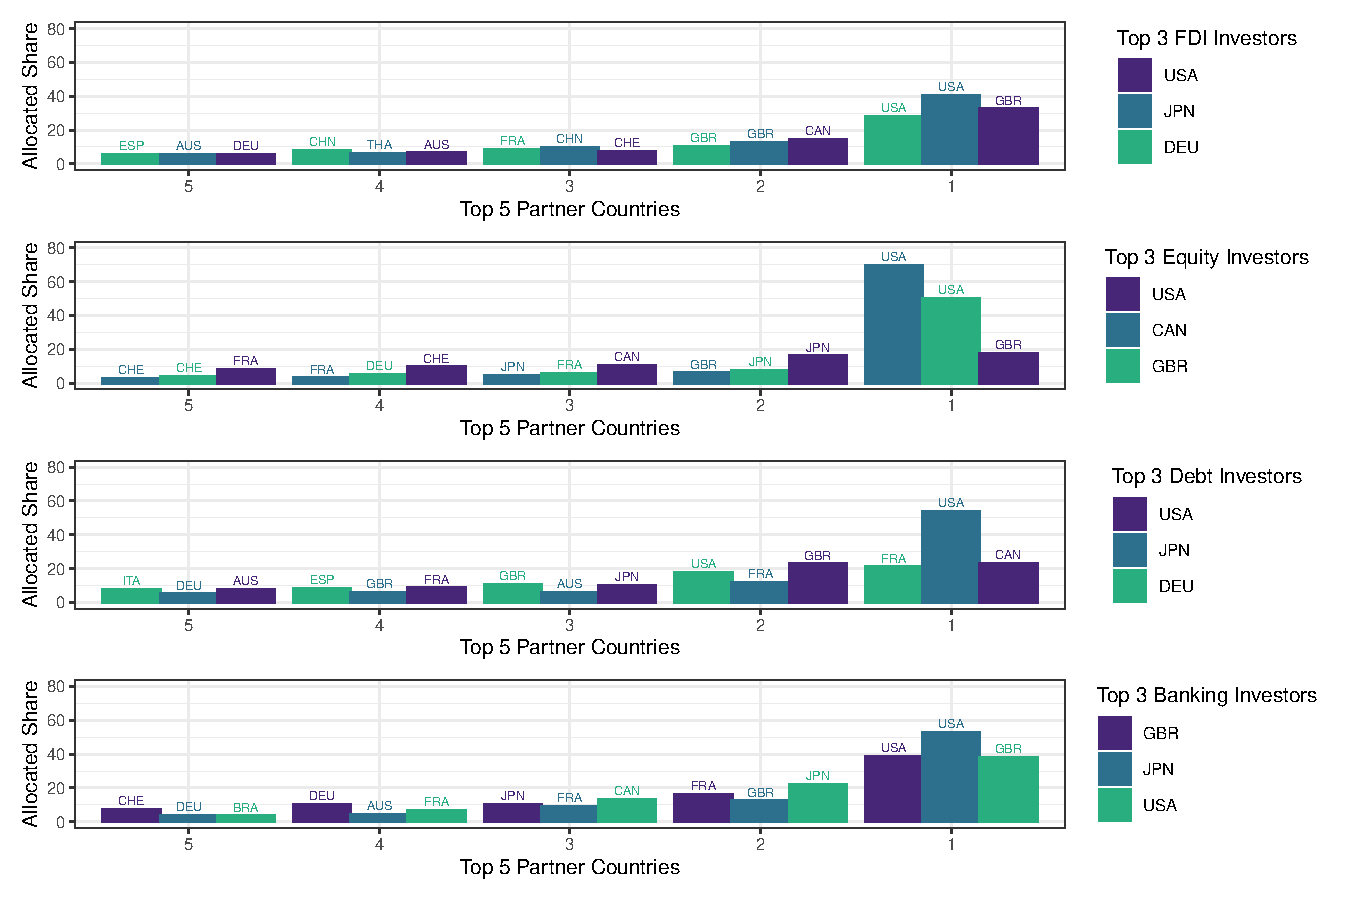
\includegraphics[width=1.1\textwidth]{Figures/fig_top3top5_bar_share_2019.pdf} 
\end{figure} 

\subsection{Playground 2: Alexandra}
Hello, what's going on? Hello Marius, how do you want to solve the conflict?

\subsection{Playground 3: Sukanya}

\subsection{Playground 4: Alessandro}

\subsection{Playground 5: Gloria}
:)
:)
$4+3=7$
test test
\subsection{Playground 6: Berta}

\subsection{Playground 7: Lukas}
Consider a small open economy subject to random exogenous shocks in its primary export sector. Let \( Y_t \) denote GDP at time \( t \), with the stochastic process 

\[
Y_t = A_t K_t^\alpha L_t^{1-\alpha},
\]

where \( A_t \) is total factor productivity (TFP), \( K_t \) is capital, and \( L_t \) is labor. Now, suppose TFP evolves according to a bizarrely specific rule: 

\[
A_t = A_{t-1} e^{\varepsilon_t}, \quad \text{where } \varepsilon_t \sim \mathcal{N}(\mu, \sigma^2) + \zeta \sin(\pi t).
\]

The inclusion of \( \zeta \sin(\pi t) \) introduces cyclical "weirdness," perhaps reflecting the influence of periodic alien invasions (or central bank interventions that feel like it). Importantly, these shocks disrupt not only production but also the cognitive coherence of economic agents, modeled by a random walk in their discount rate 

\[
\beta_t = \beta_{t-1} + \eta_t, \quad \text{with } \eta_t \sim \mathcal{N}(0, \nu^2).
\]

This setup implies that investment dynamics follow a path of chaotic determinism, as agents struggle to reconcile long-term optimization with their short-term confusion. Empirical validation requires an unprecedented dataset, preferably involving extraterrestrial phenomena or an unusually experimental central bank.

This I wrote on my local machine. Does this work?


\subsection{Playground 8: Marie}

Using git is a learning curve, but it is nice to have a good workflow once you get it. 

\subsection{Playground 9}
Hello everyone!
\subsection{Playground 10}




\section{Conflict provocation}
Conflicts may arise when working with colleagues on one common project. The following section contains five paragraphs, which the participants will be asked to change simultaneously in order to provoke conflicts!

\subsection{Conflict 1}
Economics is a powerful discipline that helps us understand resource allocation and market operations. The IWH has significantly contributed through studies on the economic effects of structural change in Eastern Germany, offering valuable insights for similar regions.
Hello what is going on. Probieren wir es mal etwas anders.
Hello what is going on. Hello, again, what is going on?

\subsection{Conflict 2}
Economics informs public policy by analyzing data and developing models. IWH researchers have influenced policy debates on labor market reforms and fiscal federalism, helping shape policies that promote economic growth and social welfare.

\subsection{Conflict 3}
Addressing global challenges like poverty and climate change, economics offers evidence-based recommendations. The IWH's research on climate change economics emphasizes the benefits of sustainable development and the need for international cooperation.

\subsection{Conflict 4}
Economics is interdisciplinary, incorporating insights from psychology and sociology to understand human behavior. The IWH fosters collaboration between economists and other experts, leading to innovative research on social networks and cultural factors.

"The history of the inflation forecasting literature is one of apparently stable relationships falling apart upon publication".

KILL ME!

\subsection{Conflict 5}
As a field that is exposed to technological change, economics continually evolves to address new challenges. The IWH pioneers research on the digital economy and technological change, providing insights into taking advantage of digitalization benefits while mitigating risks.


\end{document}
